\documentclass{uc3mpracticas}

\usepackage{helvet}
\usepackage{multicol}
\renewcommand{\familydefault}{\sfdefault}
\usepackage{changepage}
\usepackage{geometry}
\usepackage{caption}
\usepackage{xcolor,colortbl}
\usepackage{makecell}

\usepackage{amsfonts}

\definecolor{Gray}{gray}{0.85}
\definecolor{LightCyan}{rgb}{0.88,1,1}
\definecolor{LightGreen}{rgb}{0.29,1,0.39}

\newcolumntype{g}{>{\columncolor{Gray}}l}
\newcolumntype{b}{>{\columncolor{LightCyan}}c}


%%%%%%%%%%%%%%%%%%%%%%%%%%%%%%%%%%%%%%%%%%%%%%%%%%%%%%%%%%%%%%%%%%%%%%%%%%%%%%%%
%%%                   Plantilla Prácticas UC3M                               %%%
%%%                Universidad Carlos III de Madrid                          %%%
%%%                   Alejandro Valverde Mahou                               %%%
%%%%%%%%%%%%%%%%%%%%%%%%%%%%%%%%%%%%%%%%%%%%%%%%%%%%%%%%%%%%%%%%%%%%%%%%%%%%%%%%

%Permitir cabeceras y pie de páginas personalizados
\pagestyle{fancy}

%Path por defecto de las imágenes
\graphicspath{ {./images/} }

%Declarar formato de encabezado y pie de página de las páginas del documento
\fancypagestyle{doc}{
  %Cabecera
  \headerpr[1]{Test de Primalidad - AKS}{Hito 1}{Teoría Avanzada de la Computación}
  %Pie de Página
  \footerpr{}{\textbf{UC3M}}{{\thepage} de \pageref{LastPage}}
}

%Declarar formato de encabezado y pie del título e indice
\fancypagestyle{titu}{%
  %Cabecera
  \headerpr{}{}{}
  %Pie de Página
  \footerpr{}{}{}
}


\appto\frontmatter{\pagestyle{titu}}
\appto\mainmatter{\pagestyle{doc}}


\begin{document}
  %Comienzo formato título
  \frontmatter


  %Portada 1 (Centrado todo)
  \centeredtitle{Images/LogoUC3M.png}{Grado en Ingeniería Informática}{Curso 2020/2021}{Teoría Avanzada de la Computación}{Test de Primalidad - \textit{AKS}}{Hito 1}

  \vspace{55mm}

  \authors{Iván Miguelez García}{100383387}{Alba Reinders Sánchez}{100383444}{Alejandro Valverde Mahou}{100383383}{}{}

  \newpage

  %Índice
  \tableofcontents

  \newpage

  %Comienzo formato documento general
  \mainmatter


  \section{Hito 1: Heurísticas iniciales}

Para esta primera parte de la práctica se pide realizar un estudio analítico y empírico de las dos primeras heurísticas del algoritmo AKS, utilizado para determinar la primalidad de un número natural.

\vspace{2mm}

Además, se ha replicado el código en el lenguaje de programación \textit{Python} de manera alternativa, para facilitar la comprensión y análisis del código.


\subsection{Heurística 1: comprobación potencia perfecta}

Comprobar si un número es una potencia perfecta es comprobar lo siguiente:

$$ a^b = n \; | \; a \in \mathbb{N}, \; b>1$$

Si esta propiedad se cumple, se dice que $n$ no es un número primo.


\subsubsection{Estudio analítico}
Se pretende determinar la complejidad temporal de los pasos del algoritmo en los que se lleva a cabo esta primera tarea. A continuación, se realiza el estudio analítico para averiguar \textit{T(n)} y \textit{O(n)}.

\vspace{2mm}

Para ello se tiene que analizar la estructura del código. Se puede ver que está compuesto por dos bucles \textit{do while}. El bucle exterior itera sobre $a$ y el bucle interior itera sobre $b$.

\vspace{2mm}

Para el análisis del bucle exterior, es necesario determinar el valor máximo de $a$.
Se puede afirmar que, dado que el valor mínimo de $b$ es 2, el valor máximo de $a$ será $\sqrt{n}$, porque:

$$ a^2 = n \; \Rightarrow \; a = \sqrt{n} $$

El bucle interior requiere un desarrollo un poco mayor. Para conseguir el valor máximo de $b$ es necesario despejarlo en la ecuación.

\vspace{2mm}

$$ a^b = n \; \Rightarrow \; \log_a(a^b) = \log_a(n)  \; \Rightarrow \; b*\log_a(a) = \log_a(n)$$

$$ b = \log_a(n) $$

Por tanto, el número de ciclos del bucle interior depende tanto de $n$ como de $a$.

\vspace{2mm}

Si se unen ambas complejidades, se puede ver que para esta primera heurística, la complejidad temporal es:

$$ T(n) = \displaystyle \sum_{a=2}^{\sqrt{n}} \log_a(n)$$

$$ O(n) = \sqrt{n} * \log(n)$$


\subsubsection{Estudio empírico}\label{empirico}

Como se puede ver en la Figura \ref{fig:h1}, los tiempos obtenidos no coinciden con la complejidad esperada. Esto puede deberse a diversos factores.

\begin{itemize}
  \item Puede ser que no se hayan probado con números suficientemente grandes como para apreciar la curva esperada.
  \item Puede que el resultado esperado no esté escalado correctamente, y por tanto los valores no coincidan.
  \item Debido a que se ha ejecutado un código en \textit{Java} en una máquina \textit{Windows}, puede que los tiempos no estén bien medidos y tengan mucho ruido,
\end{itemize}

Para próximos hitos se volverá a probar, pero con una cantidad de números mayor.

\begin{figure}[!h]
  \centering
  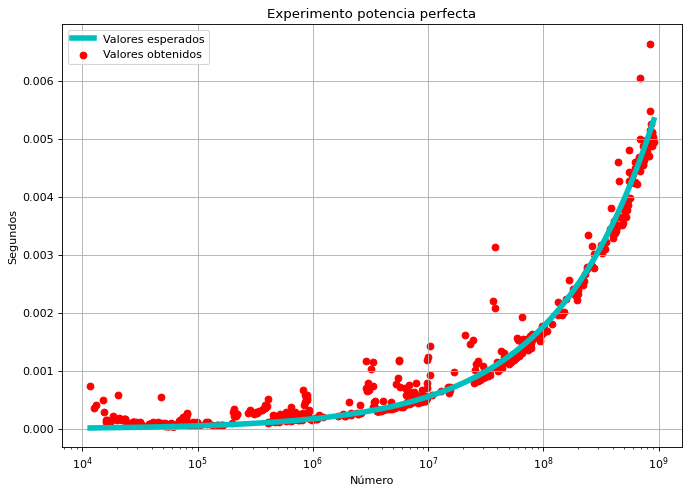
\includegraphics[width=.8\linewidth]{./Images/h1.png}
  \caption{Gráfica de tiempo de la Heurística 1}
  \label{fig:h1}
\end{figure}



\subsection{Heurística 2: cálculo de \textit{r} y \textit{mcd}}

Se parte de la siguiente premisa:

$$ \exists a \leq r \mid 1 < mcd(n,a) < n $$

Si se cumple, se dice que $n$ es un número compuesto.


\subsubsection{Estudio analítico}
Para determinar la complejidad temporal de esta segunda tarea se tiene que dividir el estudio en dos partes. En primer lugar, se debe calcular $r$ y después calcular el $mcd$.

\vspace{4mm}

\textbf{Cálculo de $r$}

\vspace{2mm}


Analizando la estructura del código se ve que está compuesto por un bucle \textit{do while} que itera sobre $r$ y que dentro se llama a la función \textit{multiplicativeOrder()}. Esta función tiene a su vez un bucle \textit{do while} que itera sobre $k$.

\vspace{2mm}

Se tiene que $r$ es el mínimo $r$ tal que:

$$ O_r(n) > log_2^2(n) $$

Donde $O_r(n)$ es el orden de $n$ módulo $r$ y representa el menor $k$ tal que:

$$ O_r(n) = k \; \Leftrightarrow \; n^k \equiv 1 \; mod \; r$$


Se sabe cuál es el máximo $r$ por el lema 4.3 de \textit{Primes is in P}\cite{primesinp}:

$$ r \leq \lceil \log^5(n) \rceil $$

Por lo tanto se concluye que la complejidad temporal del cálculo de $r$ es la unión de las complejidades de ambos bucles:

$$ O(n) = log^5(n) * log^2(n) = log^7(n) $$

\vspace{2mm}

\textbf{Cálculo del $mcd$}

\vspace{2mm}

Por último, para la complejidad de calcular el máximo común divisor de dos número $a$ y $b$, se tiene en cuenta el peor de los casos: cuando $a$ y $b$ son números consecutivos en la sucesión de \textit{Fibonacci}.

\vspace{2mm}

En este caso, el número de iteraciones del bucle es el índice del término de la sucesión, el cual se saca con la fórmula de E.Lucas:

$$ f_n =\frac{\phi^n - (1-\phi)^n}{\sqrt{5}} $$

cuya complejidad es $ log(n) $.

\vspace{2mm}


Por tanto, la complejidad total del mcd:

$$ O(n) = log(n) * log^5(n) = \log^6(n) $$

y la fórmula de la complejidad total de la heurística 2 es de:

$$ O(n) = \log^7(n) + \log^6(n)$$




\subsubsection{Estudio empírico}

En este caso, tal como se puede ver en la Figura \ref{fig:h2}, la diferencia entre el tiempo propuesto en el estudio analítico y el empírico es mucho mayor. Esto puede indicar que los cálculos del estudio analítico no sean correctos, o puede deberse a las mismas causas que se han descrito en el anterior estudio empírico \ref{empirico}.

\begin{figure}[!h]
  \centering
  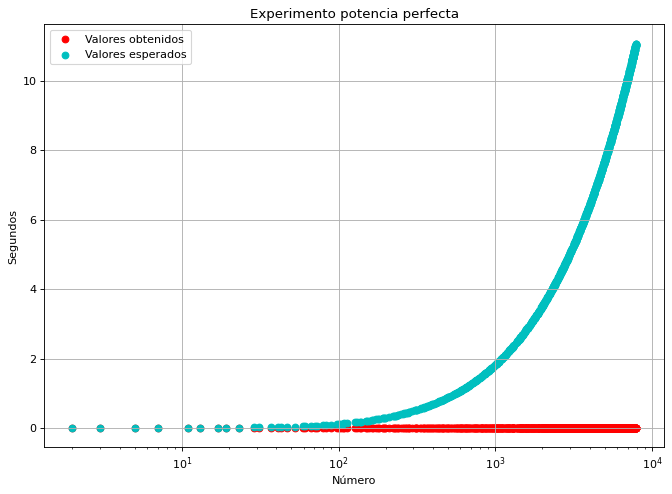
\includegraphics[width=.8\linewidth]{./Images/h2.png}
  \caption{Gráfica de tiempo de la Heurística 2}
  \label{fig:h2}
\end{figure}

\newpage

\bibliographystyle{unsrt}
\bibliography{bibliography}

\end{document}
